Los archivos relacionados a la documentación del proyecto Voorspelling se encuentran en la carpeta \textit{Documentation} del repositorio del proyecto en Github, el cual puede ser consulta en el siguiente enlace: \url{https://github.com/Noczio/VoorSpelling}. Cada directorio contiene archivos clasificados por su tipo, ya sean diagramas, formatos, flujo de la aplicación, \textit{mockups}, \textit{sketchs} y otros recursos como el cronograma del proyecto. No obstante, el documento de requerimientos es el principal para comprender el alcance del proyecto.

%requerimientos
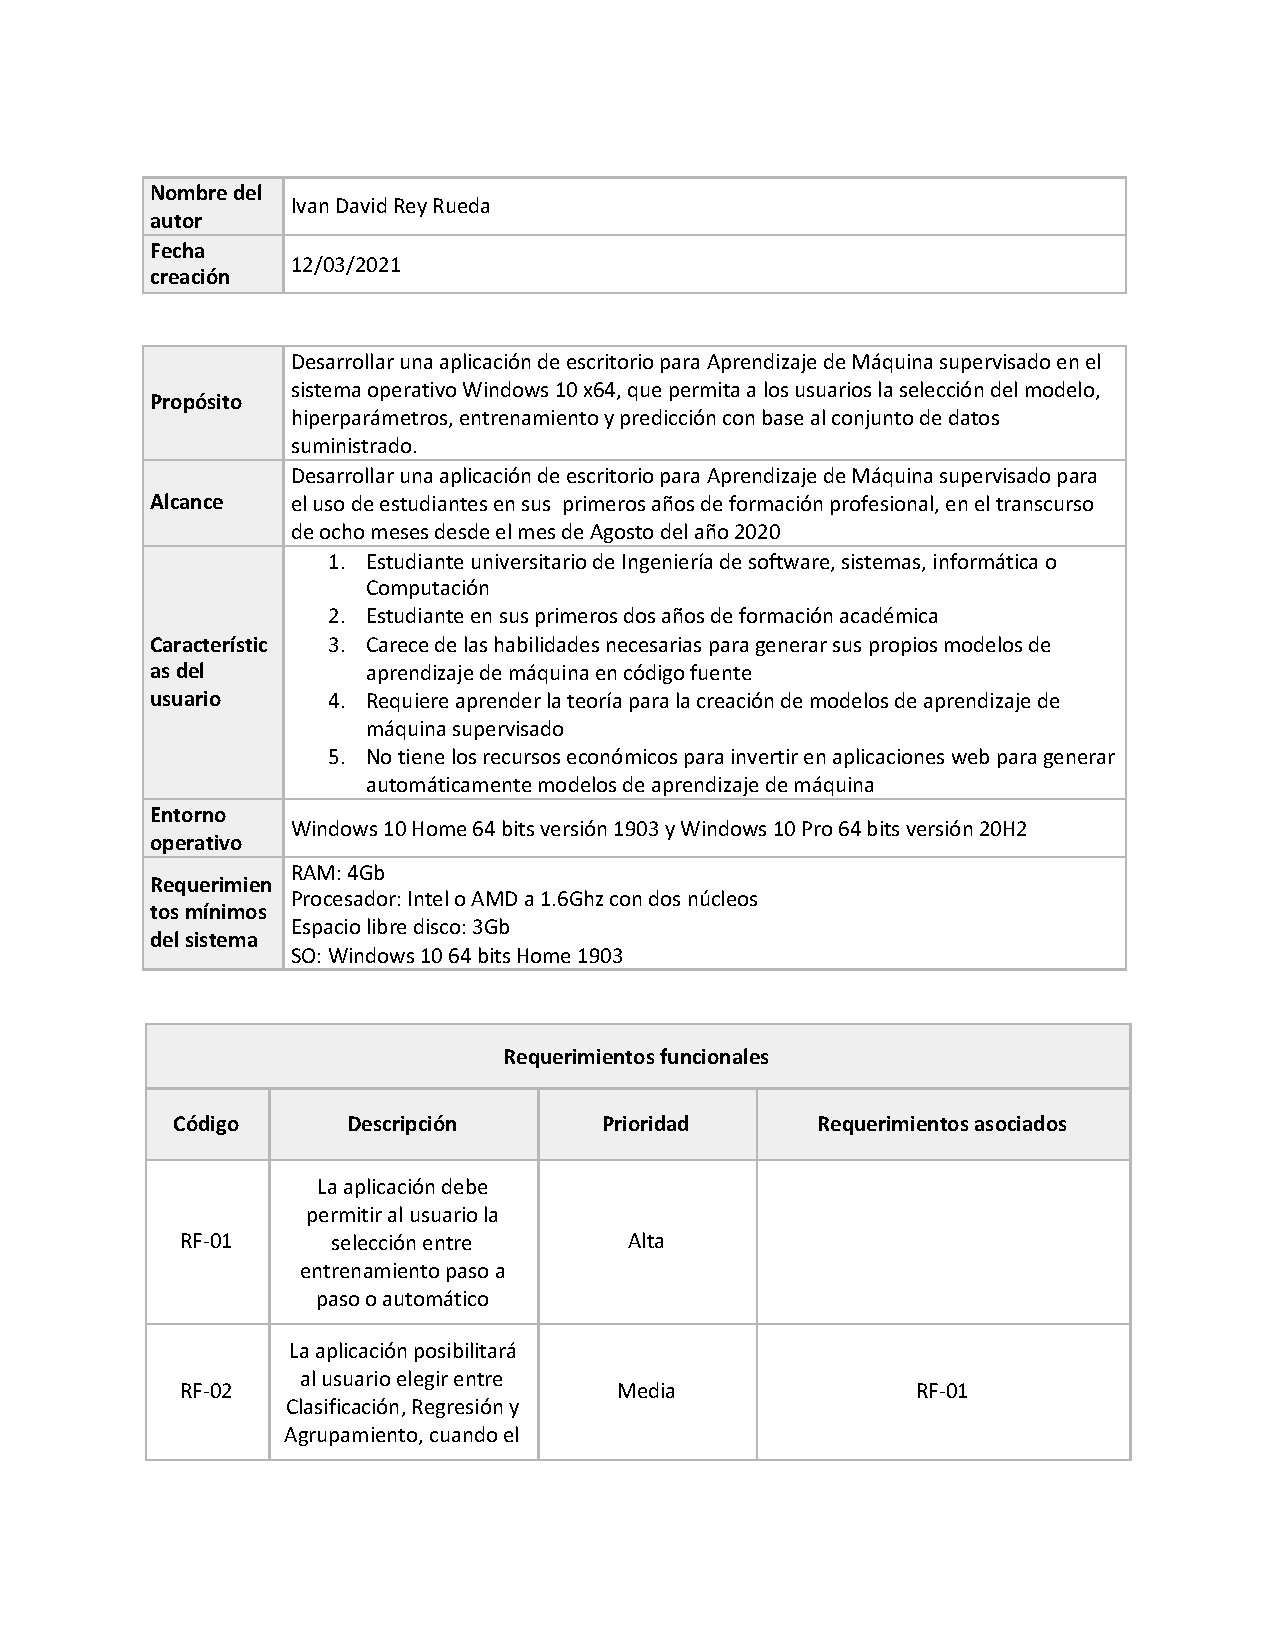
\includepdf[pages=-, pagecommand=\thispagestyle{otherplain} ,width=\textwidth]{pdfs/Requerimientos_proyecto_Firmado.pdf}